\def \supervisedLearningMethod{

    \begin{tikzpicture}

        \draw[fill=softgreen,softgreen] (2.5,0) circle [radius=2];
        \node at (2.5,0) {\Large $\xxx_i$};
        \draw[line width = 1.2cm,-{Triangle Cap[fill=softgrey]},softgrey] (5,0) to (10,0);
        \node at (7,0) {\Large $f_{\mathcal{M}}\qty(\xxx_i)$};
        \draw[fill=softblue,softblue] (12.5,0) circle [radius=2];
        \node at (12.5,0) {\Large $y_i$};
        
        \node at (2.5,2.5) {\textbf{Input}};
        \node at (7,2.5) {\textbf{Modelling}};
        \node at (12.5,2.5) {\textbf{Output}};   
    \end{tikzpicture}

}


\def \modelComplexityPlot {

    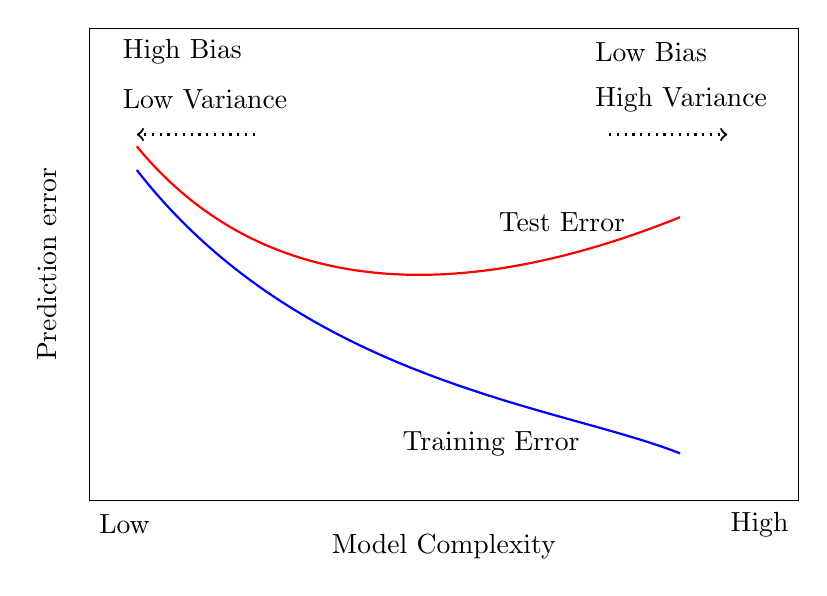
\begin{tikzpicture}[scale=3]
        \draw[] (0,0) rectangle (3,2);
        \draw[red, thick] (0.2,1.5) .. controls (0.9,0.65) and (2,1) .. (2.5,1.2);
        \draw[blue, thick] (0.2,1.4) .. controls (0.9,0.5) and (2,0.4) .. (2.5,0.2);
        \draw[->, dotted, thick] (0.7,1.55)--(0.2,1.55);
        \draw[->, dotted, thick] (2.2,1.55)--(2.7,1.55);
        \node[anchor=south] at (2,1.1) {Test Error};
        \node[anchor=south] at (1.7,0.15) {Training Error};
        \node[anchor=west] at (2.1,1.9) {Low Bias};
        \node[anchor=west] at (2.1,1.7) {High Variance};
        \node[anchor=west] at (0.1,1.9) {High Bias};
        \node[anchor=west] at (0.1,1.7) {Low Variance};
        \node[anchor=west] at (0,-0.1) {Low};
        \node[anchor=east] at (3,-0.1) {High};
        \node[anchor=south, rotate= 90] at (-0.1,1) {Prediction error};
        \node[anchor=north] at (1.5,-0.1) {Model Complexity};
    \end{tikzpicture}

}


\def \threeFoldCV{

    \begin{tikzpicture}
    
        %First line
        \filldraw[draw=softblue, fill=softblue] (0,3.5) rectangle (12,4.5);
        % third line
        \filldraw[draw=softblue, fill=softblue] (0,2) rectangle (12,3);
        \filldraw[draw=softgrey, fill=softgrey] (0,2) rectangle (4,3);
        %fourth line
        \filldraw[draw=softblue, fill=softblue] (0,0.5) rectangle (12,1.5);
        \filldraw[draw=softgrey, fill=softgrey] (4,0.5) rectangle (8,1.5);
        %fith line
        \filldraw[draw=softblue, fill=softblue] (0,-1) rectangle (12,0);
        \filldraw[draw=softgrey, fill=softgrey] (8,-1) rectangle (12,0);
        %Legend
        \node[] at (6,4) {$N$};
        
        \node[] at (2,2.5) {$\dfrac{1}{3}N$ };
        \node[] at (8,2.5) {$\dfrac{2}{3}N$ };
        
        \filldraw[draw=softblue, fill=softblue] (0,5) rectangle (0.5,5.5);
        \node[anchor=west] at (0.5,5.25) {Training data};
        
        \filldraw[draw=softgrey, fill=softgrey] (9.5,5) rectangle (10,5.5);
        \node[anchor=west] at (10,5.25) {Test data};
        
        
    \end{tikzpicture}

}


\def \QTandML{
        \begin{tikzpicture}

        \filldraw[fill=softblue, draw=softblue,ultra thick, rounded corners=15pt, opacity=0.5 ] (-3.5,0.5) rectangle (3.5,2);
        \filldraw[fill=softblue, draw=softblue,ultra thick, rounded corners=15pt, opacity=0.5] (-3.5,-2) rectangle (3.5,-0.5);
        \filldraw[fill=softblue, draw=softblue,ultra thick, rounded corners=15pt, opacity=0.5] (-3.5,-4.5) rectangle (3.5,-3);
        \draw[ultra thick,->, rounded corners=15pt] (3.5,-3.75)--(4.5,-3.75)--(4.5,1.25)--(3.5,1.25);
        \draw[->, ultra thick] (0,0.5)--(0,-0.5);
        \draw[->, ultra thick] (0,-2)--(0,-3);
        
        \node[] at (0,1.25) {Systems of interest (SOI)};
        
        \node[] at (0, -1.25) {Data to be used for ML};
        \node[] at (0,-3.75) {ML model for predictions, $\hat{y}$};
        \node[anchor=south east] at (0,-0.5) {QM computation};
        \node[anchor=south east] at (0,-3) {ML algorithm};
        \node[anchor=west] at (4.5,-1.25) {\rotatebox[origin=c]{270}{Supplementary understanding of SOI}};
    \end{tikzpicture}

}


\def \algoTLCV {%


\begin{algorithmic}[0]
\Require{$K_1$ folds in outer loop for estimation of the generalization error}
\Require{$K_2$ folds in inner loop for model selection}
\Require{$S$ models to cross-validate: $\mathcal{M}_1 , ... , \mathcal{M}_S$}
\Ensure{$\hat{E}_{\mathcal{M}*}^{\mathrm{gen}}$}

\For{$i =1,...,K_1$}
    \State{\emph{Outer CV loop. The data set, $\calD$ is split into $K_1$ folds} }
    \State{The $i$'th split of $\calD$ is $\calD_{i}^{\mathrm{par}},\calD_{i}^{\mathrm{test}}$}
    \For{$j=1,...,K_2$}
        \State{\emph{Inner CV loop doing $K_2$ splits for model selection testing $S$ models}}
        \State{The $j$'th split of $\calD_i^{\mathrm{par}}$ is $\calDss{j}{train},\calDss{j}{val}$} 
        \For{$s=1,...,S$}
            \State{Train $\mathcal{M}_s$ on $\calDss{j}{train}$ }
            \State{Let $\EMss{_{s,j}}{val}$ be the \emph{validation error} of the model $\mathcal{M}_s$ when it is \emph{tested} on $\calDss{j}{val}$}
        \EndFor
    \EndFor    
    \State{For each $s$ compute $\hat{E}_s^{\mathrm{gen}}= \sum_{j=1}^{K_2} \frac{\abs{\calDss{j}{val}}}{\calDss{i}{par}} \EMss{_s,j}{val}$ }
    \State{Select the optimal model $\mathcal{M}^*$ = $\mathcal{M}_{s^*}$ where $s^* = \argmin_s \hat{E}_s^{\mathrm{gen}}$}
    \State{Train $\mathcal{M}^*$ on $\calDss{i}{par}$}
    \State{Let $E_i^{\mathrm{test}}$ be the \emph{test error} of the model $\mathcal{M}^*$ when it is tested on $\calDss{i}{test}$}
\EndFor
\State{Compute the estimate of the generalization error: $\hat{E}^{\mathrm{gen}} = \sum_{i}^{K_1} \frac{\abs{\calDss{i}{test}}}{N} E_i^{\mathrm{test}}$}
\end{algorithmic}
% 
}


\def \lassoGeo {%

        \begin{tikzpicture}[scale=1]
            \begin{axis}[no markers,xlabel=$\hat{w}_1$, 
                ylabel=$\hat{w}_2$,
                ticks=none,
                axis x line=center,
                axis y line=center,
                ymin=-1.0,
                xmin=-1.0,
                xmax=2,
                ymax=3,
                axis equal]
                \addplot+[fill=softblue, color=softblue, opacity=0.5] coordinates
                {(-1,0) (0,1) (1,0) (0,-1)}--cycle;
            \end{axis}    
                
                \draw[red] (4.3,4.6) ellipse [x radius=1, y radius=0.5, rotate=45];
                \draw[red] (4.3,4.6) ellipse [x radius=1.5, y radius=0.75, rotate=45];
                \draw[red] (4.3,4.6) ellipse [x radius=2, y radius=1, rotate=45];
                \draw[red] (4.3,4.6) ellipse [x radius=2.37, y radius=1.185, rotate=45];
                \node[] at (4.3,4.6) {$\hat{w}$};
            
            %
        \end{tikzpicture}
    %
    }

\def \ridgeGeo {%
        \begin{tikzpicture}[scale=1]
            \begin{axis}[no markers,xlabel=$\hat{w}_1$, 
                ylabel=$\hat{w}_2$,
                ticks=none,
                axis x line=center,
                axis y line=center,
                ymin=-1.0,
                xmin=-1.0,
                xmax=2,
                ymax=3,
                axis equal]
                \end{axis}
                
                \filldraw[draw=softblue, fill=softblue, opacity=0.5] (2.7,1.4) circle (1.4);
                \draw[red] (4.3,4.6) ellipse [x radius=1, y radius=0.5, rotate=45];
                \draw[red] (4.3,4.6) ellipse [x radius=1.5, y radius=0.75, rotate=45];
                \draw[red] (4.3,4.6) ellipse [x radius=2, y radius=1, rotate=45];
                \draw[red] (4.3,4.6) ellipse [x radius=2.33, y radius=1.165, rotate=45];
                \node[] at (4.3,4.6) {$\hat{w}$};
            
        \end{tikzpicture}
    %
    }
    


\pgfplotstableread[col sep=comma] {csv/single/single_1st_lassoCV_all_rs_nias.csv}\singlefirstrsnias
\pgfplotstableread[col sep=comma] {csv/single/single_1st_lassoCV_all_rs_zb.csv}\singlefirstrszb
\pgfplotstableread[col sep=comma] {csv/single/single_1st_lassoCV_all_rs_wz.csv}\singlefirstrswz

\pgfplotstableread[col sep=comma] {csv/single/single_2nd_lassoCV_all_rs_nias.csv}\singlesecondrsnias
\pgfplotstableread[col sep=comma] {csv/single/single_2nd_lassoCV_all_rs_zb.csv}\singlesecondrszb
\pgfplotstableread[col sep=comma] {csv/single/single_2nd_lassoCV_all_rs_wz.csv}\singlesecondrswz

\pgfplotstableread[col sep=comma] {csv/single/single_3rd_lassoCV_all_rs_nias.csv}\singlethirdrsnias
\pgfplotstableread[col sep=comma] {csv/single/single_3rd_lassoCV_all_rs_zb.csv}\singlethirdrszb
\pgfplotstableread[col sep=comma] {csv/single/single_3rd_lassoCV_all_rs_wz.csv}\singlethirdrswz

\pgfplotstableread[col sep=comma] {csv/single/single_4th_lassoCV_all_rs_nias.csv}\singlefourthrsnias
\pgfplotstableread[col sep=comma] {csv/single/single_4th_lassoCV_all_rs_zb.csv}\singlefourthrszb
\pgfplotstableread[col sep=comma] {csv/single/single_4th_lassoCV_all_rs_wz.csv}\singlefourthrswz


\def \Singleplot{
\begin{tikzpicture}
             \begin{axis} [xlabel={Predicted value [eV]}, 
            ylabel={Target value [eV]},
            ymax=1,
            ymin=-1,
            legend style={at={(0.95,0.2)},anchor=east}
            ]
                \addplot[color=red, mark=square*, only marks]   table[x=p,y=t, col sep=comma] \singlefourthrsnias;
                \addlegendentry{NiAs}
                
                \addplot[color=blue, mark=triangle*, only marks]   table[x=p,y=t, col sep=comma] \singlefourthrszb;
                \addlegendentry{Zb}
                \addplot[color=green!90!black, mark=*, only marks]   table[x=p,y=t, col sep=comma] \singlefourthrswz;
                \addplot[thin, black] {x};
                \addlegendentry{Wz}
            \end{axis}
        \end{tikzpicture}

}
    
\pgfplotstableread[col sep=comma] {csv/multi/multi_1st_plot_multi_lasso_ref_rs.csv}\multiffirst
\pgfplotstableread[col sep=comma] {csv/multi/multi_2nd_plot_multi_lasso_ref_rs.csv}\multisecond
\pgfplotstableread[col sep=comma] {csv/multi/multi_3rd_plot_multi_lasso_ref_rs.csv}\multithird
\pgfplotstableread[col sep=comma] {csv/multi/multi_4th_plot_multi_lasso_ref_rs.csv}\multifourth


\def \Multiplot{
\begin{tikzpicture}
             \begin{axis} [xlabel={Predicted value [eV]}, 
            ylabel={Target value [eV]},
            ymax=1,
            ymin=-1,
            axis equal,
            legend style={at={(0.95,0.2)},anchor=east}
            ]
                \addplot[color=red, mark=square*, only marks]   table[x=p1,y=t1, col sep=comma] \multifourth;
                \addlegendentry{NiAs}
                
                \addplot[color=blue, mark=triangle*, only marks]   table[x=p2,y=t2, col sep=comma] \multifourth;
                \addlegendentry{Zb}
                \addplot[color=green!90!black, mark=*, only marks]   table[x=p3,y=t3, col sep=comma] \multifourth;
                \addplot[thin, black] {x};
                \addlegendentry{Wz}
            \end{axis}
        \end{tikzpicture}
}
    
\pgfplotstableread[col sep=comma] {csv/implicit/big_1st_lassoCV_all_rs.csv}\bigfirst
\pgfplotstableread[col sep=comma] {csv/implicit/big_2nd_lassoCV_all_rs.csv}\bigsecond
\pgfplotstableread[col sep=comma] {csv/implicit/big_3rd_lassoCV_all_rs.csv}\bigthird
\pgfplotstableread[col sep=comma] {csv/implicit/big_4rd_lassoCV_all_rs.csv}\bigfourth

\def \Implicitplot{
\begin{tikzpicture}
             \begin{axis} [xlabel={Predicted value [eV]}, 
            ylabel={Target value [eV]},
            ymax=1,
            ymin=-1,
            legend style={at={(0.95,0.2)},anchor=east}
            ]
                \addplot[color=red, mark=square*, only marks]   table[x=p1,y=t1, col sep=comma] \bigfourth;
                \addlegendentry{NiAs}
                
                \addplot[color=blue, mark=triangle*, only marks]   table[x=p2,y=t2, col sep=comma] \bigfourth;
                \addlegendentry{Zb}
                \addplot[color=green!90!black, mark=*, only marks]   table[x=p3,y=t3, col sep=comma] \bigfourth;
                \addplot[thin, black] {x};
                \addlegendentry{Wz}
            \end{axis}
        \end{tikzpicture}

}
  
  
\def \featureiterations{
    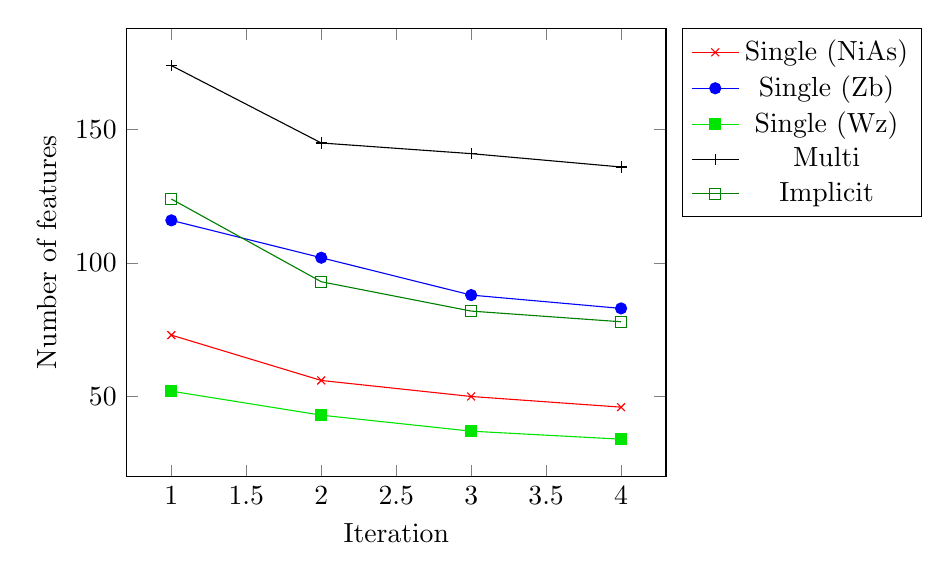
\begin{tikzpicture}
        \begin{axis}[
        xlabel={Iteration},
        ylabel={Number of features},
        %legend style={at={(1,0.5)}},
        legend pos=outer north east,
        ]
            \addplot[color=red,mark=x] coordinates {
	        (1,   73 )
	        (2,   56)
	        (3,   50)
	        (4,   46)
            };
            \addlegendentry{Single (NiAs)}
            \addplot[color=blue,mark=*] coordinates {
	        (1,   116)
	        (2,   102)
	        (3,   88)
	        (4,   83)
            };
            \addlegendentry{Single (Zb)}
            \addplot[color=green!90!black,mark=square*] coordinates {
	        (1,   52 )
	        (2,   43)
	        (3,   37)
	        (4,   34)
            };
           \addlegendentry{Single (Wz)}
            \addplot[color=black,mark=+] coordinates {
	        (1,   174)
	        (2,   145)
	        (3,   141)
	        (4,   136)
            };
            \addlegendentry{Multi}
            \addplot[color=green!50!black,mark=square] coordinates {
	        (1,   124)
	        (2,   93)
	        (3,   82)
	        (4,   78)
            };
            \addlegendentry{Implicit}

            
            
            
        \end{axis}
    \end{tikzpicture}   
}
   
    